\section{Build a twisted bilayer}\label{sec:twisted-structures}
\index{Twisted bilayers}
\index{Moire superlattices@Moiré superlattices}

\subsection{From a relative rotation to a common period}

Place two graphene monolayers on top of each other and rotate one about the surface normal. Their local registry then varies across the plane: in some regions atoms nearly coincide vertically, while elsewhere an atom in one layer lies near the center of a hexagon in the other. Viewed over a larger area, these local arrangements form a repeating moiré pattern.

A periodic calculation also needs a common cell. Simply rotating the upper layer within its original small cell generally leaves the two layers incompatible across the boundaries. \ui{Twist Moiré Superlattice} selects an integer supercell for each layer so that both fit a shared in-plane period. The target angle guides the search, while a particular set of integer relations defines the resulting model.

The first example is a graphene bilayer twisted by approximately $21.7868^\circ$. Its relatively short common period gives only 28 carbon sites, making the layers and cell easy to inspect. Complete this example before trying smaller angles to understand how angle, period, and model size are related.

\subsection{Prepare the two layers}

The tool uses hexagonal in-plane primitive cells: the two in-plane vectors have equal lengths and enclose $60^\circ$ or $120^\circ$. Each input graphene monolayer here contains two C sites, has an in-plane lattice constant of $2.46\,\text{\AA}$, and a box height of $15\,\text{\AA}$. It is periodic in both in-plane directions and nonperiodic along the normal.

The supplied \file{twist-graphene-bottom.json} and \file{twist-graphene-top.json} come from the same monolayer input, with the same geometry as \file{graphene-layer.json} used earlier. Separate filenames identify their roles in the project; they do not mean that a relative rotation has already been applied.

\begin{steps}
  \item Import both JSON files into one project and name the structures \file{twist-bottom} and \file{twist-top}.
  \item Open the bottom layer's 3D document and check that it has two model sites. More than two atoms may be displayed to show periodic connections.
  \item Inspect the lattice: both in-plane lengths should be $2.46\,\text{\AA}$ and their angle approximately $120^\circ$. Check that the top layer has the same lattice and composition.
  \item Activate \file{twist-bottom}. On \ui{Crystal Modeling}, open \ui{Interface Modeling} in \ui{Surfaces \& Interfaces}, then choose \ui{Twist Moiré Superlattice}.
  \item Select \file{twist-top} under \ui{Top-layer structure}. Choose an existing project structure rather than entering a disk path.
\end{steps}

Begin with these two original monolayers. Keep any bilayer created by insertion or stacking separately; it is no longer a single input layer for this exercise.

\subsection{Enter a small-model parameter set}

\begin{table}[htbp]
\centering
\caption{Parameters for the 28-site twisted graphene bilayer.}
\begin{tabularx}{\linewidth}{lX}
\toprule
Parameter & Input and meaning\\
\midrule
Top-layer structure & Select \file{twist-top}.\\
Angle (degrees) & Enter \literalinput{21.786789} as the target relative angle.\\
Interlayer gap (Å) & Enter 3.35 for the initial separation between layers.\\
Total vacuum thickness (Å) & Enter 15 for the total empty height outside the slab.\\
Maximum in-plane strain & Enter 0.03, or 3\%.\\
Maximum atom count & Enter 200 as the upper limit on total model sites.\\
Maximum coincidence index & Enter 6 to bound the integer matching search.\\
\bottomrule
\end{tabularx}
\end{table}

\ui{Angle (degrees)} is a numeric field; enter the value without a degree symbol. \ui{Interlayer gap (Å)} and \ui{Total vacuum thickness (Å)} are also numerical lengths. Maximum strain is a fraction: 0.03 means 3\%; entering 3 would specify a different requirement.

The atom limit does not request exactly 200 atoms. Likewise, \ui{Maximum coincidence index} limits the search over integer coincidence relations; it does not simply repeat a direction six times. Within the search bounds, the tool considers angle error, strain, and model size and selects an integer match. These limits therefore differ from the three repeat factors in \ui{Build Supercell}.

This command selects one match internally. Unlike \ui{Stack Heterostructure}, it has no candidate ranking or candidate-index field. Check the actual size and relative orientation after construction. To compare other matches, retain the original layers and generate and save separate results for each parameter set.

\begin{steps}
  \item Enter the table's values and click \ui{Preview}. The two-site monolayer should become a larger periodic structure containing two layers.
  \item Look nearly along the surface normal and check that the hexagons in the two layers are rotated relative to each other. Inspect the side view to confirm that there are still only two layers, with no unintended atoms between them.
  \item Check for 28 model sites. The expanded in-plane cell may display more atoms because of periodic images.
  \item Apply, name the result \file{graphene-twist-21p786789}, and save the project. Retain both monolayers so later comparisons can start from the same inputs.
\end{steps}

\begin{figure}[!htb]
\centering
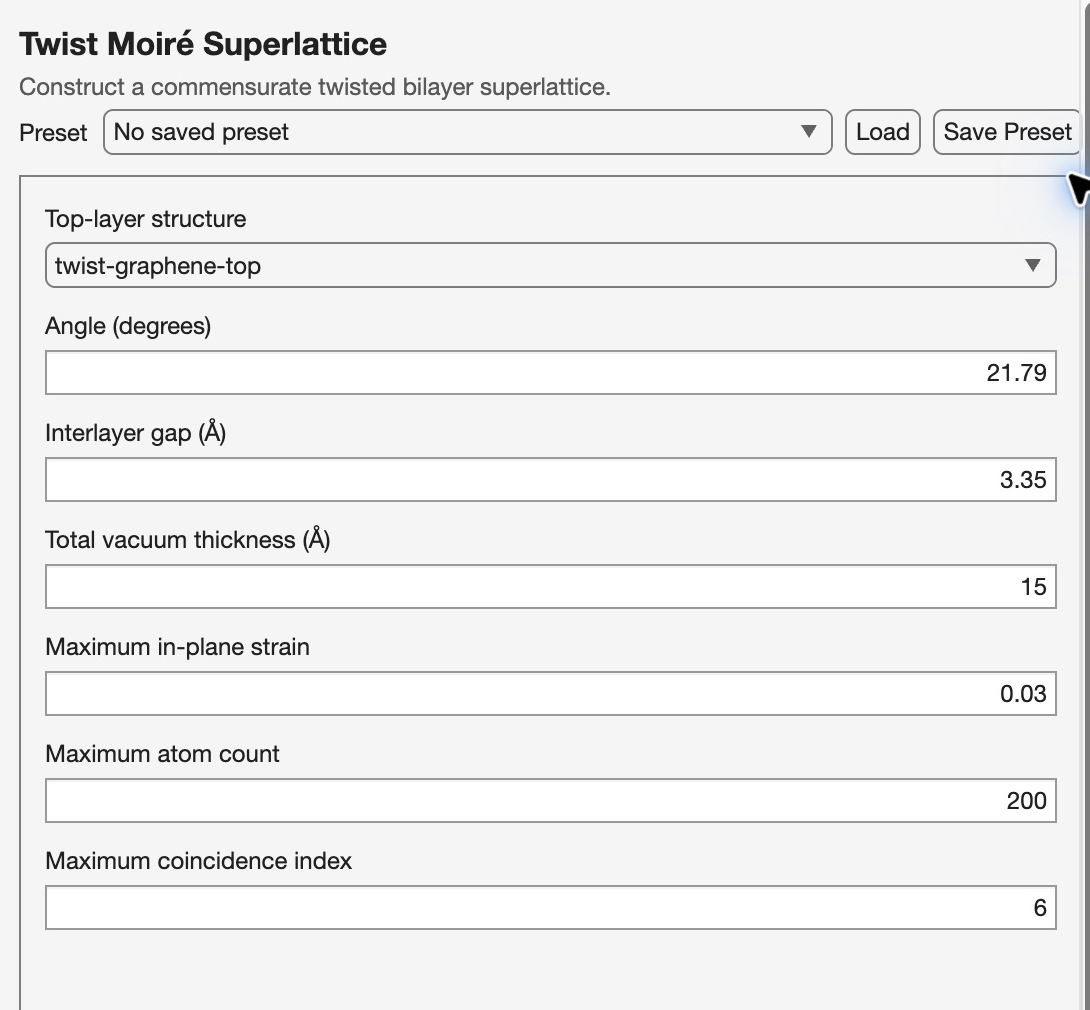
\includegraphics[width=107mm]{publication-assets/crop-7c221ceb9a35fdad53a3.png}
\par\vspace{2mm}

\includegraphics[width=107mm]{publication-assets/crop-faecdf5879e359505e34.png}
\caption{Twist parameters and preview. The entered target is 21.786789 degrees; after the field loses focus, it displays 21.79 at the available precision. The top layer retains its imported name, \file{twist-graphene-top}, corresponding to \file{twist-top} in the instructions. The preview contains 28 sites.}
\label{fig:online-twist-parameters}
\end{figure}

\begin{figure}[!htb]
\centering
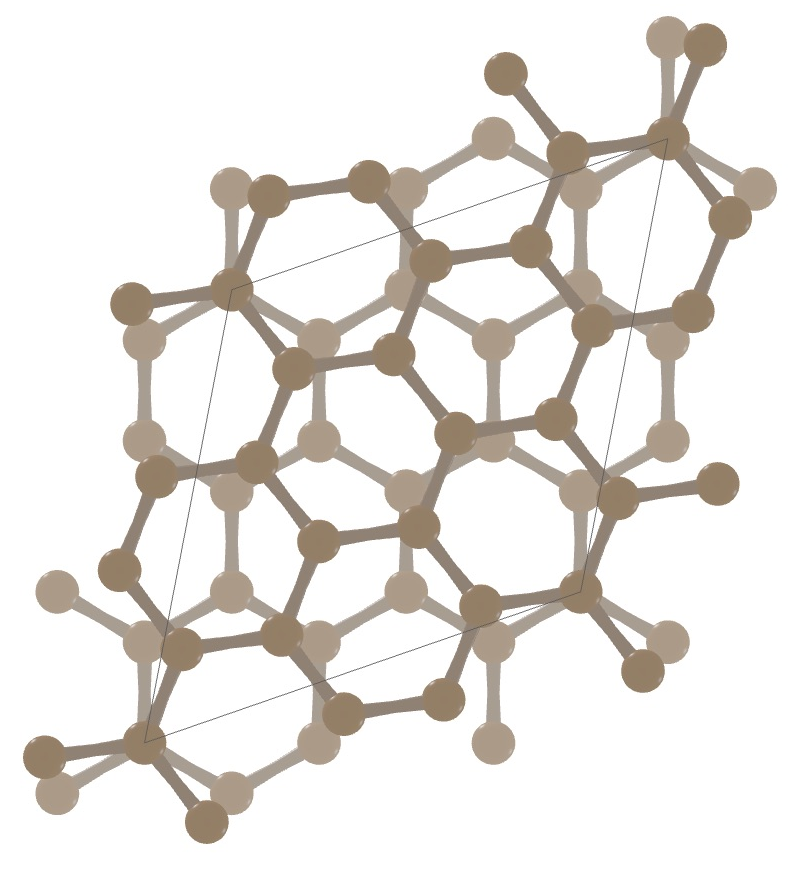
\includegraphics[width=93mm]{publication-assets/crop-89eb072a4598add87b05.png}
\caption{View along the normal of the twisted graphene bilayer. The hexagons are rotated relative to one another. The 28 model sites appear as 68 displayed atoms at the current periodic display range.}
\label{fig:online-twist-top}
\end{figure}

\subsection{Interpret the generated cell}

The supplied \file{graphene-twist-21p786789.json} is the reference structure generated with these parameters; a CIF with the same base name is provided for geometry exchange. The model contains 28 C sites, 14 in each layer. Each layer's in-plane area is seven times that of the original two-site monolayer.

Both in-plane vectors are approximately $6.508548\,\text{\AA}$ long, giving an area of approximately $36.6859\,\text{\AA}^2$. The new cell angle is $60^\circ$, whereas the input primitive cell uses $120^\circ$. These are different lattice-basis representations; the angle change alone does not establish that the crystal has been distorted. Check lengths, area, site count, and periodic connectivity together.

For these graphene inputs, the period length can also be checked as $\sqrt{7}\times2.46\,\text{\AA}$, or approximately $0.651\,\mathrm{nm}$. This is the common cell's in-plane repeat length, not the interlayer separation or a C--C bond length. Each layer retains a shortest nearest-neighbor distance of approximately $1.420282\,\text{\AA}$, matching the input monolayer.

The side view shows a layer separation of $3.35\,\text{\AA}$ and a normal cell height of $18.35\,\text{\AA}$. Each layer is planar here, so the cell height is the layer separation plus the total vacuum. Total vacuum of $15\,\text{\AA}$ means all empty height outside the slab, not $15\,\text{\AA}$ on each side.

\begin{figure}[!htb]
\centering
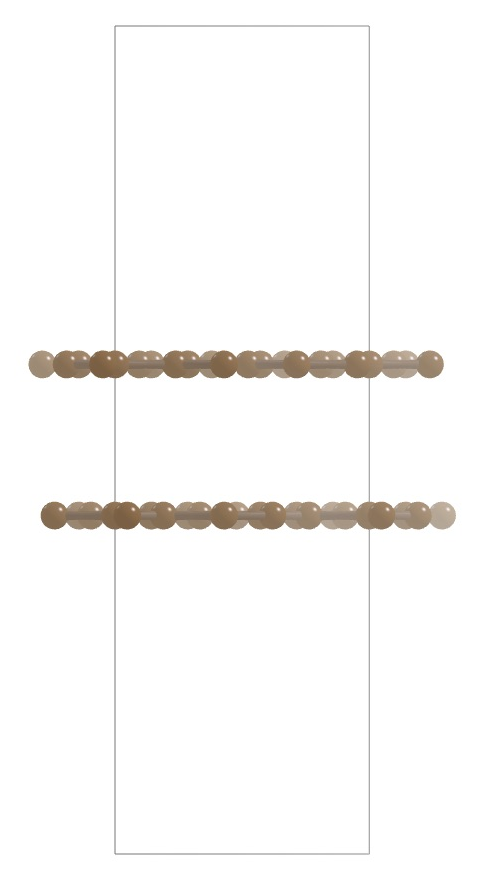
\includegraphics[width=67mm]{publication-assets/crop-a8d161a93e2745b16ef3.png}
\caption{Side view of the same model. The two atomic planes and the cell boundaries distinguish the interlayer gap from the external vacuum.}
\label{fig:online-twist-side}
\end{figure}

The reference model's achieved angle is $21.786789298^\circ$, approximately $2.98\times10^{-7}$ degrees from the target, with zero in-plane strain. The relative angle can also be obtained from nearest-neighbor bond directions in the two layers.

Exact matching information is stored in the \file{moire} section under \file{properties} in the native JSON. Open the JSON in a text editor and search for \file{achieved_angle_degrees}. The fields \file{target_angle_degrees}, \file{angle_error_degrees}, and \file{in_plane_strain} record the target, angle error, and in-plane strain. For your own structures, choose \ui{Export file → Structure file}, then export JSON. Do not choose \ui{Scene JSON}: it records the viewing scene rather than the structural matching information.

\subsection{Why the achieved angle may differ from the target}

Target angles range from $0^\circ$ to $60^\circ$. Using hexagonal in-plane symmetry, the tool represents achieved matching angles between $0^\circ$ and $30^\circ$. Apply that convention when comparing larger targets. The example stays within the smaller range so that target and achieved values can be compared directly.

A common period requires particular integer relations. An arbitrary decimal angle need not have a reasonably sized periodic cell that matches it exactly. Changing the target to $22^\circ$ while retaining the other settings still gives 28 sites and an achieved angle of approximately $21.786789298^\circ$, now with an error of approximately $0.213211^\circ$.

The two constructions have the same final geometry but different target inputs. The supplied \file{graphene-twist-target22.json} preserves the second result for comparison. Report the achieved angle rather than using only the target entered in the parameter dialog.

\begin{table}[htbp]
\centering
\caption{Effects of target angle and size limits for these inputs.}
\begin{tabularx}{\linewidth}{lX}
\toprule
Input change & Actual result\\
\midrule
Target $21.786789^\circ$, limit 200 & 28 sites; achieved angle approximately $21.786789298^\circ$.\\
Target $22^\circ$, limit 200 & The same 28-site geometry and achieved angle; error approximately $0.213211^\circ$.\\
Target $21.786789^\circ$, limit 24 & A four-site match close to $0^\circ$, missing the original target.\\
\bottomrule
\end{tabularx}
\end{table}

The third case shows why successful construction and an acceptable angle match are separate checks. Once the 28-site match is excluded by the limit of 24, the tool selects from the remaining search space. If the resulting size differs markedly from your expectation, check the parameters and achieved angle together before increasing the search bounds.

Smaller twist angles generally require longer common periods and more atoms. To compare angles, first hold layer spacing and strain requirements fixed, then gradually increase the allowed size and maximum coincidence index. This reveals whether the broader search improves the angle match or merely produces a larger structure. The approximately $21.8^\circ$ example uses small integers and is a useful starting point for learning the procedure and checking periodicity.

\subsection{Choose an assembly tool for your purpose}

The \ui{Interface Modeling} menu groups several assembly methods. Decide which geometric relationships are already known and which ones the tool should find.

\begin{table}[htbp]
\centering
\caption{Choosing insertion, lattice matching, or twist construction.}
\begin{tabularx}{\linewidth}{lX}
\toprule
Tool & Suitable starting situation\\
\midrule
Insert Structure & The two parts already have defined positions; specify a translation and retain the current host cell.\\
Stack Heterostructure & Compare common in-plane cells using allowed strain, repetition, and rotation ranges.\\
Twist Moiré Superlattice & Start from hexagonal monolayers and a target angle, then find a common period from integer lattice relations.\\
\bottomrule
\end{tabularx}
\end{table}

In the \ui{Stack Heterostructure} candidate table, area, strain, atom count, and rotation each answer a different question. Area and atom count indicate calculation size; strain measures the change needed to match the original lattices; rotation defines their relative orientation. A low-strain candidate can be large, while the smallest-area candidate may require substantial deformation. Compare these quantities before inspecting the atomic arrangement.

The twist command instead uses hexagonal integer relations to select a common period, then assembles the layers. It does not ask for a candidate index in the same dialog. To compare targets of $21.786789^\circ$ and $22^\circ$, build each result from the two original monolayers and record them separately. Do not apply the command again to an already assembled bilayer.

Rotating the camera only changes the viewpoint; rotating selected atoms changes their positions. Neither replaces periodic matching of the shared cell. Alongside layer orientation, display the cell boundaries and inspect repetitions along both in-plane directions to ensure that the local pattern and full periodic cell describe the same model.

These tools assemble layered interfaces along the normal. An in-plane lateral heterojunction requires separate preparation of the junction's atomic arrangement and boundaries.

\subsection{Build a twisted graphene/h-\headinglatin{BN} heterostructure}

Twisting also applies to layers of different materials. The earlier zero-angle graphene/h-BN match illustrates how different in-plane lattice constants are accommodated. A relative rotation can be introduced as well. Here graphene is the bottom layer with lattice constant $2.46\,\text{\AA}$, and h-BN is the top layer with $2.50\,\text{\AA}$.

\begin{steps}
  \item Import \file{twist-graphene-bottom.json} and \file{hBN-layer.json} afresh, naming them \file{graphene-bottom} and \file{hBN-top}. Do not use the previously twisted bilayer as the bottom layer.
  \item Activate the new graphene monolayer. In \ui{Twist Moiré Superlattice}, choose \file{hBN-top} under \ui{Top-layer structure}.
  \item Retain the table's target angle, layer separation, total vacuum, 200-site limit, and maximum coincidence index of 6. Keep maximum in-plane strain at 0.03.
  \item Preview and check for $\mathrm{C_{14}B_7N_7}$ with 28 total sites. Each layer has 14 sites, but their elements differ.
  \item Apply and save as \file{graphene-hBN-twist-21p786789}, then compare with the zero-angle \file{graphene-hBN-stacked.json}.
\end{steps}

The achieved angle is again approximately $21.786789298^\circ$. The principal in-plane strain is 0.016, or 1.6\%. The h-BN dimensions are matched to the common graphene lattice, while separation remains $3.35\,\text{\AA}$ and normal cell height remains $18.35\,\text{\AA}$. Strain changes dimensions; twist changes relative orientation. They describe different modifications.

Both construction commands produce geometric models. To study interfacial charge transfer, band alignment, or junction properties, build the appropriate calculations on the saved structures and distinguish the input layer separation from the distance obtained after calculation.

\subsection{Save twisted models}

A project retains the input layers, generated structures, and later workflows. JSON and CIF are supplied for structure exchange. JSON preserves in-plane/normal periodicity flags, layer indices, and twist-matching metadata. CIF is used to exchange the cell and atomic positions. These CIF files are imported as periodic in all three directions, and moiré metadata must be retained separately. Prefer JSON for further 2D modeling comparisons here. When using CIF in another calculation, check normal boundary conditions and vacuum for the target method.

\begin{steps}
  \item Give each result a name identifying the material, achieved angle, and main change, such as ``graphene bilayer, achieved angle 21.7868 degrees,'' rather than a generic \file{result}.
  \item Record the input lattices, target and achieved angles, strain, layer separation, total vacuum, site count, and in-plane period. Use a separate comparison-table column for each quantity.
  \item Reopen the saved project and check both layers' composition and the cell. Keep the parameter record with an exported structure so its geometry can be interpreted in other software.
  \item To regenerate the examples, start MATLAB\regmark{} with \file{-nojvm}, configure the toolbox path, and run \file{twist_examples.m} from the supplied examples directory. To check saved files only, run \file{verify_twist_examples.m}.
\end{steps}

The supplied structures are starting models for relaxation and electronic structure calculations. When comparing twist effects, use consistent functionals, pseudopotentials, cutoffs, and suitable sampling, and save those settings with the structures.
